\chapter{Market Survey}
The following products are available which provide similar fuctionality to our system

\section{Workscape}

Product Website: 
\url{www.workscape.io/products/manage/smart-sensors/}
\newline
Device White Paper: 
\url{https://goo.gl/K2D8hQ}

\vspace{10pt}

Workscape\cite{workscape} provides sensing devices similar to ours. It also provides meeting room booking and scheduling applications for mobile devices.
Workscape provides the booking and scheduling applications indepedantly or it also provides the applications along with the devices.
It also uses the data generated by the sensors to provide analytics on room occupancy status over a period of time.
The solutions offered by workscape are similar the ones proposed by us.

Workscape follows a subscricption pricing policy as follows
\begin{itemize}
\item Basic: 8\textdollar \hspace{1pt} per room per month which includes Calendar sync Room display app, Mobile App, Web booking, Reporting and analytics
\item Sensor: 15\textdollar \hspace{1pt} per room per month which includes Everything in Basic + Smart sensors + Room automation + Enhanced reporting and analytics
\end{itemize}

The "Sensor" solution costs 15\textdollar  \hspace{1pt} per room per month which would equal to 2700\textdollar \hspace{1pt} for 15 rooms per year

\vspace{10pt}

\begin{center}
	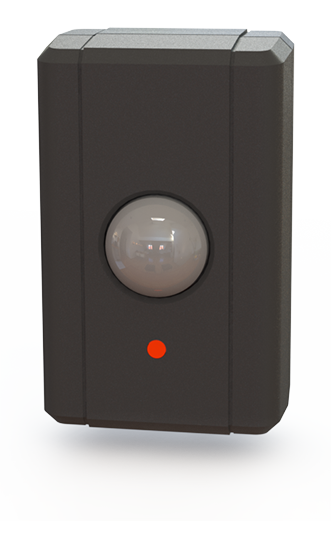
\includegraphics[scale=0.27]{Workscape1.png}
	\hspace{40pt}
	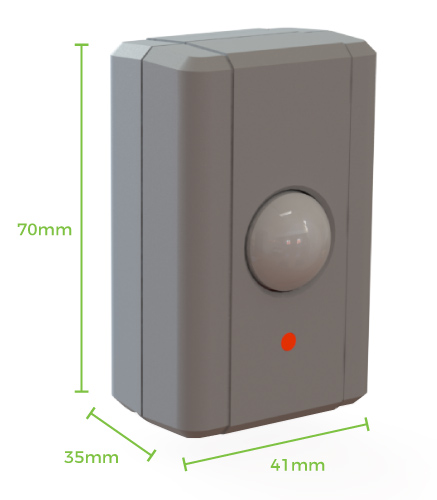
\includegraphics[scale=.55]{Workscape2.png}
\end{center}

\section{OccupEye}

Product Website:
\url{https://www.occupeye.com/}
\newline
Product Whitepaper: 
\url{https://goo.gl/PpC2pw}

\vspace{10pt}

Similar to workscape, occupeye can also moniter the occupancy status of a room. In addition occupeye is also intended to serve as a workstation occupancy monitoring sensor.
OccupEye\cite{occupeye} is targeted towards improving the workspace utilization.
Like our proposed solution all the sensors transmit to a central receiving station which then pushes the data to the Internet. OccupEye analytics is web-based portal that can generate analytics on room/workspace utilization. This can help enable dynamic workspace allocation and serve to promote efficient workspace utilization.

\begin{figure}[ht]
\begin{center}
	
\vspace{20pt}
	
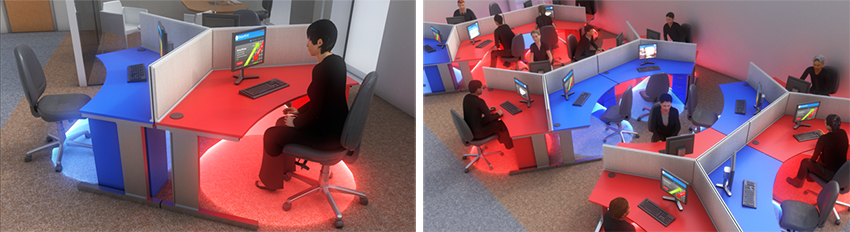
\includegraphics[scale=0.25]{HotColdDeskOccupEye.png}
\caption{Workstation occupancy monitoring: Hot/Cold desk}

\vspace{40pt}

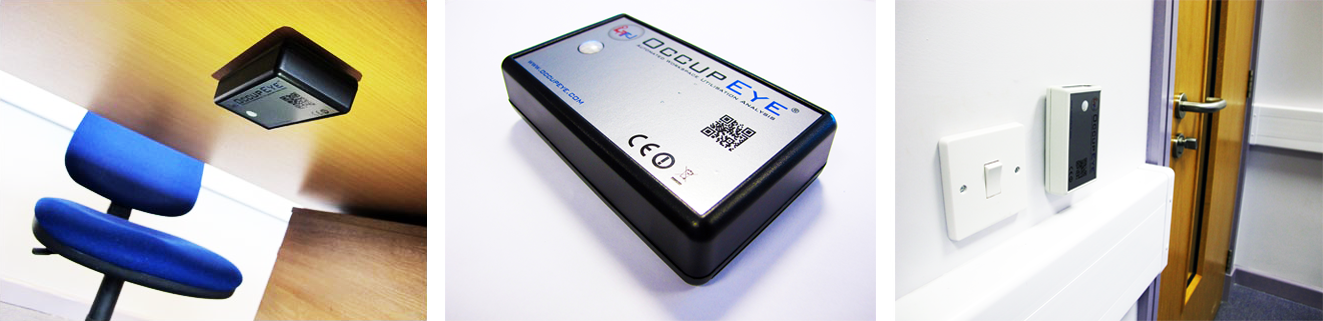
\includegraphics[scale=0.25]{OccupEyedeployment.png}
\caption{Workstation/room occupancy sensing}

\vspace{40pt}

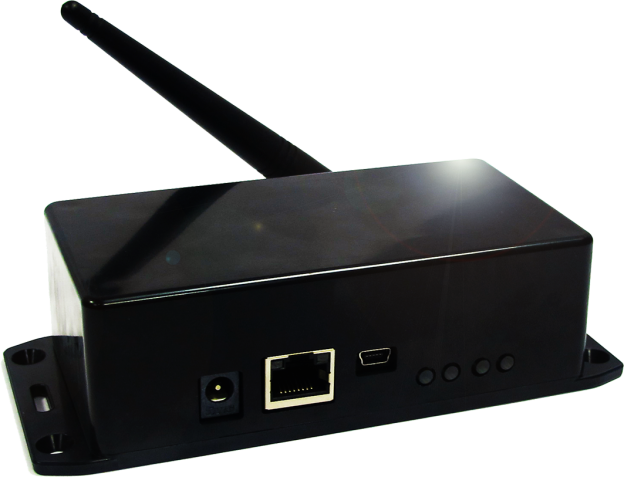
\includegraphics[scale=0.25]{OccupEyeReceiver.png}
\caption{Base station}

\end{center}
\end{figure}	